\documentclass[a4paper, 12pt]{book}

\usepackage{setspace}
\doublespacing
%\setstretch{1.7}
%\linespread{1}

\usepackage{indentfirst}
%\usepackage{lastpage}

\usepackage{graphicx}
\usepackage{subfigure}
\graphicspath{{images/}}
\DeclareGraphicsExtensions{.PNG, .png}
%\DeclareGraphicsRule{.psc}{eps}{}{}
%\DeclareGraphicsRule{*}{PNG}{}{}
\graphicspath{{./}{../../../images/}{./images/}}   % Give paths as required


\usepackage[a4paper]{geometry}
\geometry{left=2.0cm}
\geometry{top=2cm}
\geometry{bottom=2.5cm}
\geometry{right=2cm}

\usepackage{makeidx}
\makeindex

\usepackage{glossary}
\makeglossary

\usepackage[pdftex]{hyperref}
\hypersetup{colorlinks,
                        citecolor=blue,
                        filecolor=blue,
                        linkcolor=blue,
                        urlcolor=blue}

%\newcommand{\subscript}[1]{\ensuremath{_\textrm{#1}}}
\newcommand{\highlight}[1]{\textbf{\Huge{$\mathfrak{#1}$}}}
\newcommand{\commenth}[1]{\textbf{\emph{#1}}}

\usepackage{amsmath,amsthm,amssymb}
\usepackage[mathcal]{eucal}

%\usepackage{amsmath}
\usepackage{multirow}
\usepackage{listing}
\usepackage[subfigure]{tocloft}

% ===== definition of the command \citazione{text}{author} =====
\newcommand{\citeyours}[2]
{
 \vspace*{-0.8cm}
 \hfill%
 \begin{minipage}{0.5\textwidth}
 \flushright
 ``\small\textit{#1}``
 \\\vspace*{0.1cm}{\normalfont#2}
 \end{minipage}
 \vspace*{0.6cm}
}

%%===== header & footer =====
%\usepackage{fancyhdr}
%\pagestyle{fancy}
%\renewcommand{\chaptermark}[1]{\markboth{\thechapter\ #1}{}}
%\renewcommand{\sectionmark}[1]{\markright{\thesection\ #1}}
%\fancyhf{}
%%\fancyhead[LE,RO]{\bfseries\thepage}
%\fancyhead[LO]{\bfseries\rightmark}
%\fancyhead[RE]{\bfseries\leftmark}
%\renewcommand{\headrulewidth}{0.5pt}
%\addtolength{\headheight}{2pt}
%\fancypagestyle{plain}{
%        \fancyhead{}
%        \renewcommand{\headrulewidth}{0pt}
%}
%\renewcommand{\footrulewidth}{0.5pt}
%\fancyfoot[C]{\bfseries\thepage}
%%\addtolength{\footheight}{2pt}
%%=================================================

%===== header & footer =====
\usepackage{fancyhdr}
\pagestyle{fancy}
\fancyhf{}
\renewcommand{\headrulewidth}{0pt}
\fancypagestyle{plain}{
        \fancyhead{}
        \renewcommand{\headrulewidth}{0pt}
}
\fancypagestyle{plain2}{
        \fancyhf{}
}
\renewcommand{\footrulewidth}{0pt}
\fancyfoot[C]{\thepage}
%=================================================

% \def\l@section{\vskip2mm\bf@dottedtocline{1}{1.5em}{2.3em}}
% \def\l@subsection{\@dottedtocline{2}{3.8em}{4.8em}}
% \def\l@subsubsection{\@dottedtocline{3}{8.6em}{4.1em}}
% 
% \def\listoffigures{\section*{\listoffiguresname\markboth
%  {\listoffiguresname}{\listoffiguresname}}\@starttoc{lof}}
% \def\l@figure{\@dottedtocline{1}{1.5em}{4.3em}}
% \def\listoftables{\section*{\listoftablesname\markboth
%  {\listoftablesname}{\listoftablesname}}\@starttoc{lot}}
%\let\l@table\l@figure

%\def\l@subsection{\@dottedtocline{2}{3.8em}{5.3em}}
%\def\l@subsubsection{\@dottedtocline{3}{3.8em}{3.2em}}

%\def\l@figure{\@dottedtocline{(1)}{1.5em}{3.6em}}

%\renewcommand{\listfigurename}{Figures}

%\newlength{\subfiglabelskip=0pt
% \renewcommand{\thesubfigure}{\thefigure.\arabic{subfigure}}
% \makeatletter
%   \renewcommand{\p@subfigure}{}
%   \renewcommand{\@thesubfigure}{\thesubfigure:\hskip0pt}
% \makeatother

%\setcounter{lofdepth}{2}
%\setcounter{lotdepth}{2}
%
%\addtolength{\cftfignumwidth}{1em}
%\addtolength{\cftsubfigindent}{1em}
%\addtolength{\cftsubfignumwidth}{1.5em}
%
%\addtolength{\cfttabnumwidth}{1em}
%\addtolength{\cftsubtabindent}{1em}
%\addtolength{\cftsubtabnumwidth}{1.5em}
%
%\setlength{\cftsecnumwidth}{3.3em}
%\setlength{\cftsubsecindent}{4.8em}
%\setlength{\cftsubsecnumwidth}{4.2em}


\begin{document}

\thispagestyle{empty}
\include{FrontPage}
\thispagestyle{empty}
\cleardoublepage

\thispagestyle{empty}
\include{Copyright}
\thispagestyle{empty}
\cleardoublepage

\pagenumbering{roman}


%\frontmatter
\phantomsection
\addcontentsline{toc}{chapter}{Front Page}
\begin{titlepage}
\noindent
\begin{center}
\vspace*{0.5mm}
{{\large{Thesis Title}}}

\vspace{1cm}

\large{A dissertation submitted in partial fulfillment of the requirements for the degree of Master of Science/Doctor of Philosophy at Indian Institute of Science Education and Research Bhopal}

\vspace{4cm}

\large{by}\\
\vspace{0.5cm}
\large{Your Name}\\
\begin{large}
{MSc/MTech/ME, Institute Name (Year)}\\
{BS/BTech/BE, Institute Name (Year)}\\
\vspace{1.5cm}
Advisor: Dr. Kuntal Roy\\
Electrical Engineering and Computer Sceince (EECS) Department
\end{large}

\vspace{3cm}
\begin{large}
Indian Institute of Science Education and Research Bhopal\\
Bhopal, Madhya Pradesh, India\\
Date
\end{large}
\end{center}

\end{titlepage}
\cleardoublepage

\setstretch{1}
\phantomsection
\addcontentsline{toc}{chapter}{Contents}
\tableofcontents
\cleardoublepage

\phantomsection
\addcontentsline{toc}{chapter}{List of Figures}
\listoffigures
\cleardoublepage

\phantomsection
\addcontentsline{toc}{chapter}{List of Tables}
\listoftables
\cleardoublepage
%\setstretch{1}

\thispagestyle{plain2}
\phantomsection
\addcontentsline{toc}{chapter}{Abstract}
\vspace*{0.5mm}
\begin{center}
\large{Abstract}
\end{center}

\vspace*{1cm}
\begin{flushleft}
Title: TITLE
\end{flushleft}

\begin{flushleft}
By Your Name
\end{flushleft}

\begin{flushleft}
A dissertation submitted in partial fulfillment of the requirements for the degree of Master of Science/Doctor of Philosophy at Indian Institute of Science Education and Research Bhopal 
\end{flushleft}

\begin{center}
Indian Institute of Science Education and Research Bhopal, Year.
\end{center}

\begin{center}
Advisor: Dr. Kuntal Roy, Electrical Engineering and Computer Sceince (EECS) Department
\end{center}

\vspace*{1cm}
\doublespacing
Write abstract of your thesis

\cleardoublepage

%\newpage \clearpage
\newpage \pagenumbering{arabic}

\chapter{Introduction}
\label{ch:introduction}

\highlight{I}n this chapter, we will introduce Energy-Efficient Neuromorphic Computing. Neuromorphic computing or brain-inspired computing is a way to mimic biological brain processing. Artificial neural network models the biological neural network. The biological neural network is a collection of interconnected neurons, A typical biological neuron consists of Dendrites, Soma, and Axon. Where each neuron receives signals from other neurons through dendrites and sends signals to other connected neurons through the axon. Soma is the functional unit of a neuron, the main process soma deals with is the accumulation of signals received through dendrites, and to activate the neuron. In general, a neuron can be in two states, Firing (activated state) or non-firing (deactivated) state. When a neuron sends output to other neurons, then the neuron is said to be in a firing state or in a non-firing state. The state of a neuron is decided by the incoming signals: if the summation of the input signals is more than a certain threshold, then the neuron is in an activated state, else it is in a deactivated state. In a similar fashion, the Artificial Neural Network (ANN) is modeled, which will be described in the upcoming sections. The demand for ANN is increasing tremendously. The number of applications of ANN is skyrocketing, some of the important applications to point out are Self-driving cars, Face recognition, Face detection, and Virtual assistants like Google Assistant, Siri, etc. Which uses a massive amount of neuromorphic computing. Usually, neuromorphic computing is performed on transistor-based devices. We aim to use spintronic devices which can be more energy-efficient than the traditional transistor-based devices. Apart from this, spintronic devices have some inherent advantages over transistor-based devices, like Weight, Sum, and Threshold function comes in-built, and spintronic devices are non-volatile in nature.

\section{Artifical Neural Network (ANN)}
Similar to a biological neural network, Artificial Neural Network is a collection of interconnected artificial neurons (or nodes). Like the biological counterpart, the artificial neuron takes multiple inputs, where each input is collected by the neuron through the edges, each edge has its own strength known as Weight. Each neuron has a summation block, an activation block, and a bias term. All the weighted inputs received by the artificial neuron and the bias term is at first sent into the summation block. The output of the summation block is fed into the activation block. The output of the activation block is the final output of the neuron. The weight and the bias term are the optimizing parameters of an ANN. It's a two-phase process, Training, and Evaluation. In the training phase, the neural network (NN) is trained on training data. Training data is a tuple (X, T), where X is the input and T is the desired output (or target). The training data is fed into the NN, the model learns the underlying feature of the data, and optimizes its weight and biases, so as to obtain a minimum error. Then comes the evaluation phase, in this phase, the trained NN is used to obtain the output for those inputs, which was never used in the training phase.
\subsection{Architecture}
We already stated that ANN is a system of interconnected neurons, but there is a specific architecture, by which the neurons are connected to each other. First of all, a NN consists of three layers: Input Layer, Hidden Layers, Output Layer

Input Layer:
This layer serves as the interface where the input to the NN is given by the user.

Output Layer:
This layer serves as the interface where the output from the NN is given to the user.

Hidden Layers:
The Hidden layer is not just one single layer like the Input and the Output Layer, this layer exists between the input layer and output layer where the majority of the computation of NN happens. Since the user does not interact with this layer, hence it is termed as the hidden layer.

Each layer consists of several neurons, based on the type of layer. The Input layer and the Output layer, the no. of neurons in these layers are decided by the problem at hand. Based on the problem requirement, these numbers are set. On the other hand, there is no particular rule for setting the number of neurons in hidden layers. In fact, the no. of hidden layers and the no. of neurons inside each layer are set during the training phase. 

The way the neurons are connected to each other is as follows:
The output of each neuron is connected to all other neurons in the next layer
There are no self-loops or feedback loops

\subsection{Activation Function}
Technically the activation function is a non-linear mathematical function. The activation function reflects the property of activation of a neuron in a biological NN. In ANN, similar to the biological NN, the neurons would not transmit signals to the next connected neuron unless a certain threshold is reached. The threshold is set by the bias component of a neuron. The most simplistic activation function, which also prevails in the biological NN is a step function, 
EQN 1
But generally in ANN, we use a much smoother version of the step activation function known as the Sigmoid activation function.
EQN 2
Often in the case of Deep Neural Networks, there may be millions-millions of neurons,  using the sigmoid function as an activation function will make it computationally expensive, hence another activation function is used known as Rectilinear Unit Function (ReLu). We will see in backpropagation why using ReLu will give more computational advantage over other activation functions.

\subsection{Forward Propagation}
In Forward-propagation, we need to set our neural architecture, after which the input traverses from the input layer to the output layer through the hidden layers. The weight and bias terms have already been configured. Here is an example: we have taken a very simple ANN with one neuron in the input layer, one in the output layer, and one hidden layer which consists of one neuron. With weights as W1 and W2, for edges connecting node 1 with 2 and node 2 with 3 respectively. X is the input given to the NN and Y is the output received from the NN. Node 2 and node 3 have the bias term B2 and B3 respectively. The following figure describes the neural architecture.

[fig of simple NN, in MID term press backup, slide 15]

Generally, the input node does not have any bias term; it's just a simple node, which accepts input and sends it to its subsequent connected node. 
Forward propagation steps:
Output from node 1, X
X travels through the edge of strength W1, hence the input received at node 2 is XW1, Z1=XW1
Node 2 processes the input (iz. Summation and activation) and gives the output, Z2=sigma(Z1 + B2) =sigma(X.W1 + B2)
Z2 travels through the edge of strength W2, hence the input received at node 3 is Z2.W2, Z3=Z2.W2
Node 3 process the input Z3, and gives the output, Y=sigma(Z3 +B3)=sigma( sigma(X.W1 + B2).W2+B3)
Which is the final output of the NN
\subsection{Gradient Descent}
We previously saw that ANN trains itself by minimizing error on changing the weight and biases. Gradient descent is an approach to do so. 
[fig mid term slide 16]
In the figure, we have Error in the y-axis and optimizing parameter K in the x-axis. K can be a weight or a bias term. Since weight and the bias term are the optimizing parameters of the NN, our goal is to choose such a value of K where the error becomes minimum. At first, we start at some initial point (initial K value), the initial point is chosen randomly, why it is chosen randomly will be explained shortly. The slope at that point is computed. The slope will suggest that in which direction of K, the minimum exists and at what rate the minimum should be reached. But the slope magnitude is generally high and there is a huge chance that it will overshoot the minimum point. Hence a learning rate (LR) is multiplied by the slope. LR is usually chosen small, but not very small. The step size is defined as Slope x LR. And the new K value is defined as Knew=K-step-size. This way the K takes larger jumps when it is far away from the minimum and it takes smaller jumps near the minimum. So that it does not overshoot. 
[fig mid term slide 17]
The optimizing term is chosen randomly at the beginning, because if the error plot turns out to be like the above plot, and we always start at some fixed initial point, then there is a high chance of getting stuck in a local minimum. Hence the K is chosen randomly to begin, so as to increase the probability of not getting stuck in a local minimum. This problem is unavoidable but it can be minimized.

\subsection{Backpropagation}
Backpropagation is the process in which the weight and biases are fine-tuned so as to decrease the error. It uses gradient descent, for minimization of error. Since it is done during the training phase, we use the training data, here also using the same ANN architecture as fig in Forward propagation. For simplicity, we have omitted the bias term. For input X, we have target value T, the output received from the NN, for input X is Y.
Error = (T-Y)2
Optimizing for W1, 
EQN 4

The steps through 1-4 are repeated until we get the minimum error, similarly, it is done for all the weights and biases in the NN.

\section{Character Recognition Model}
This is an implementation of ANN, where the NN model is given a set of noisy 7x5 pixels binary patterns of an alphabet, where each pixel value can be either 0 or 1. From the input, the model recognizes the alphabet despite having noises.
Here the input is a 35 (7x5)-bit word of the test character, e.g., 
A: 01110 10001 10001 11111 10001 10001 10001
And the output is a 26-bit word suggesting the alphabet
A: 10000000000000000000000000
B: 01000000000000000000000000 and so on

\subsection{Neural Architecture}
Input layer: It has 35 neurons, as it will receive 35-pixel values
Output layer: It has 26 neurons, as it will give a 26-bit word suggesting the alphabet 
Hidden Layers: Only 1 Hidden layer and there are 40 neurons in the hidden layer


\section{Neural Network using Spintronics}
An electron along with a charge also contains spin. We can use this spin to store and transmit binary information, we can encode UP spin as 0 and DOWN spin as 1. Spintronic devices are rapidly developing nano technologies, they can store, process and communicate. This is just a matter of spin rotation, since no charge movement, there is no ohmic dissipation, but there is dissipation due to magnetization damping. In order to change the spin, we need to apply external charge voltage/current, hence there is dissipation due to that. At 100 nm dimension, all the spins align in one direction, which can be represented as one single big spin.
\subsection{Magnetic Anisotropy}
Magnetic anisotropy means magnetization is not same in all directions. The magnetization of a specimen depends on its shape. When a specimen of finite size is magnetized by an external magnetic field, the free poles which appear on its ends will produce a magnetic field directed opposite to the magnetization. This field is called the demagnetizing field. The intensity of the demagnetizing field $H_d$ is proportional to the magnetic free pole density and therefore to the magnetization
\[H_d=N_d\frac{I}{\mu_0}\]
where $N_d$ is the demagnetizing factor, which depends on the shape of the specimen.\\
In case of a sphere, because of it total symmetry, the demagnetization factor is same in all direction, hence there is no anisotropy.
In case of an ellipsoid,as it is not symmetric in all direction, anisotropy exists but because of its shape, it is difficult to fabricate in a planar wafer.
Which brings us to elliptical cylinder, it has anisotropy and because of its planar surface, it is easy to fabricate on a planar wafer. The elliptical cylinder poses the in-plane shape magnetic anisotropy. The energy of the same is given by $E=\frac{1}{2}\Omega M_s H_k sin^2 \theta$, where the $\Omega$ is the volume of the elliptical cylinder, $M_s$ is the saturation magnetization, $H_k$ is the coercive field

\subsection{Magnetic Field along in-plane: Easy and Hard axis}
\subsection{Perpendicular Anisotropy}
\subsection{Magnetostriction}
\subsection{Multiferroics and Multiferroic Composites}
In nature there exist, ferroelectric and ferromagnetic materials. Ferroelectric materials are those materials whose polarization changes on changing the electric field and vice versa, similar to this the ferromagnetic materials are those materials whose magnetization changes on changing the magnetic field and vice verse. Along with this materials, there are certain specimens which posses both the properties of ferroelectric and ferromagnetic materials. These materials are known as multiferroics. For a multiferroic material, the polarization changes on changing the magnetic field and the magnetization changes on changing the electric field.   
\subsection{Giant Magneto Resistance (GMR)}
\subsection{Tunneling Magneto Resistance (TMR)}

\section{Magnetic Thermal Annealing}
\section{Ferro-magnteic Resonance (FMR)}
When a magnetic material is placed in a DC magnetic field, the magnetization vector rotates in counter-clock wise direction, along the direction of the DC field. This is called the precessional motion of the magnetization vector, as it does, it losses energy, the rotational body falls in the direction of the DC field, this is known as damping. This precesssing of magnetization vector is captured by the   Landau-Lifshitz Equation (LL Equation):
\[\frac{dM}{dt}=-|\gamma|M\times H_{eff} - \frac{\alpha |\gamma|}{M}M\times M\times H_{eff}\]
where $\alpha$ and $\gamma$ are the damping parameter and the Gyromagnetic ratio of the magnetic material respectively.\\
In FMR experiment our aim is to find $\alpha$ of the magnetic material.\\
We will consider $\alpha$ later. The precessional motion of the magnetization vector is given by 
\[\frac{dM}{dt}=-|\gamma|M\times H_{eff}\]
DC magnetic field is applied along the z-axis, hence $M_z=M$, and the $M_x$ and $M_y$ has $e^{-i\omega t}$ dependence, hence
\[\frac{dM_x}{dt}=-|\gamma|(H_z + (N_{yy}-N_{zz})M)M_y\]
and
\[\frac{dM_y}{dt}=|\gamma|(H_z + (N_{xx}-N_{zz})M)M_x\]
Solving the above two equation, we get
\[\omega^2=|\gamma|^2(H_z + (N_{yy}-N_{zz})M)(H_z+(N_{xx}-N_{zz})M)\]
In case of, sphere: $N_{xx}=N_{yy}=N_{zz}$, therefore, $\omega =|\gamma|H_z$\\
In-plane FMR: $N_{xx}=N_{zz}=0, N_{yy}=1$, therefore, $\omega =|\gamma|\sqrt{H_z(H_z+M)}$\\
Perpendicular FMR:  $N_{xx}=N_{yy}=0, N_{zz}=1$, therefore, $\omega =|\gamma|(Hz-M)$\\
On Linearizing the small rotations,
\[\frac{d^2\phi}{dt^2}+\alpha|\gamma|M\frac{d\phi}{dt}+\omega_0^2\phi=0\]
where $\omega_0=|\gamma|\sqrt{H_z(H_z+M)}$, for IN-plane FMR\\
To negative the damping, and to keep the magnetization rotating, a transverse AC field $H_y(t)=H_{y0}e^{i\omega t}$ is applied
\[\frac{d^2\phi}{dt^2}+\alpha|\gamma|M\frac{d\phi}{dt}+\omega_0^2\phi =|\omega|^2MH_{y0}e^{i\omega t} \]
On solving the differential equation, $\phi(t)=\phi_0e^{i\omega t}=|\phi_0|e^{i(\omega t+\delta)}$, where\\
\[\phi_0=\frac{|\gamma|^2MH_{y0}}{(\omega_0^2 - \omega^2)^2 + (\alpha|\gamma|M\omega)^2}[(\omega_0^2 - \omega^2)-i\alpha|\gamma|M\omega]\]
\[|\phi_0|=\frac{|\gamma|^2MH_{y0}}{\sqrt{(\omega_0^2 - \omega^2)^2 + (\alpha|\gamma|M\omega)^2}}, tan \delta = \frac{-\alpha|\gamma|M\omega}{(\omega_0^2 - \omega^2)}\]
The FMR absorption is given by the Imag($\phi_0$), known as the Lorentzian
\[Imag(\phi_0)=\frac{|\gamma|^2MH_{y0}\alpha|\gamma|M\omega}{(\omega_0^2 - \omega^2)^2 + (\alpha|\gamma|M\omega)^2}\]
at $\omega=\omega_0$, $Imag(\phi_0)=\frac {H_{y0}|\gamma|}{\alpha \omega_0}$\\
The FMR linewidth $\Delta H$, Half width at half maximum (HWHM) is given by:
\[\Delta H =\frac{\alpha\omega_0}{|\gamma|}\]
\section{Magnetic Force Microscopy (MFM)}
\section{Piezo Force Microscopy (PFM)}
\section{Vibrating Sample Magnetometer (VSM)}
\section{X-ray Diffraction (XRD)}
\section{X-ray Reflectivity (XRR)}
\section{Strain-gauge}
\section{Stress-strain Testing Machine}
\section{Proposed Device}
\section{Experimental Apparatus}
\subsection{Spin Coater}
\begin{figure}[H]
	\centering
		
		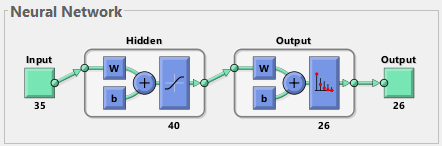
\includegraphics{4.png}
		\caption{Spin Coater}
\end{figure}
\subsection{Shaker}
\begin{figure}[H]
	\centering
		
		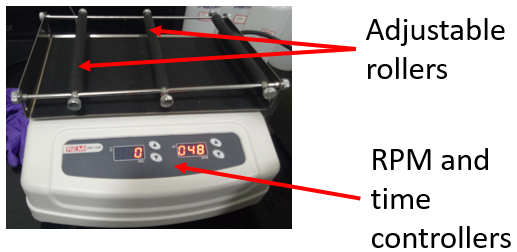
\includegraphics{5.png}
		\caption{Shaker}
\end{figure}
\subsection{Hot Plate}
\begin{figure}[H]
	\centering
		
		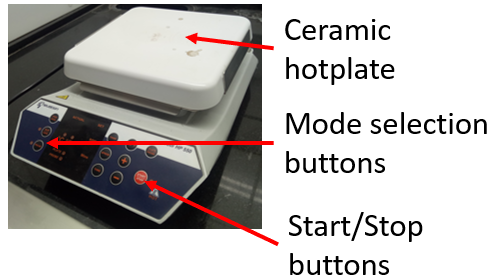
\includegraphics{6.png}
		\caption{Hot Plate}
\end{figure}
\subsection{Ultrasonic Cleaner}
\begin{figure}[H]
	\centering
		
		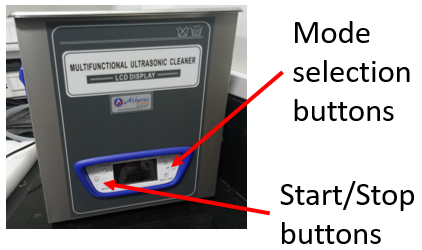
\includegraphics{7.png}
		\caption{Ultrasonic Cleaner}
\end{figure}
\subsection{Hot Air Oven}
\begin{figure}[H]
	\centering
		
		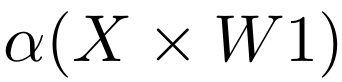
\includegraphics{8.png}
		\caption{Hot Air Oven}
\end{figure}
\subsection{Rota Mantle}
\begin{figure}[H]
	\centering
		
		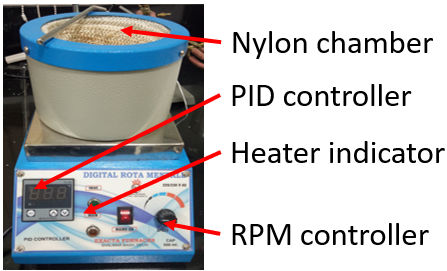
\includegraphics{9.png}
		\caption{Rota Mantle}
\end{figure}
\subsection{Nitrogrn Gun}
\begin{figure}[H]
	\centering
		
		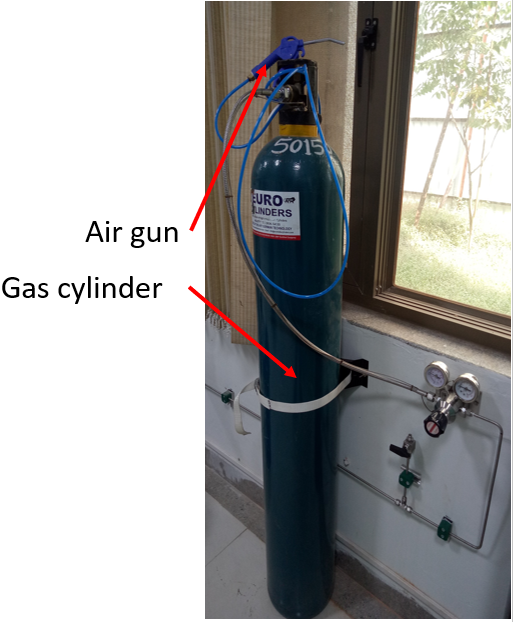
\includegraphics{10.png}
		\caption{Nitrogen Gun}
\end{figure}
\subsection{Vacuum Desiccator}
\begin{figure}[H]
	\centering
		
		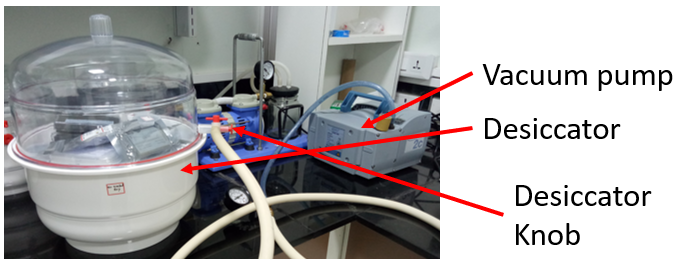
\includegraphics{11.png}
		\caption{Vacuum Desiccator}
\end{figure}
\subsection{Muffle Furnace}
\begin{figure}[H]
	\centering
		
		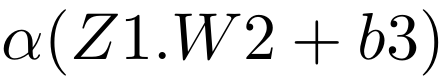
\includegraphics{12.png}
		\caption{Muffle Furnace}
\end{figure}
\subsection{Fume Hood}
\begin{figure}[H]
	\centering
		
		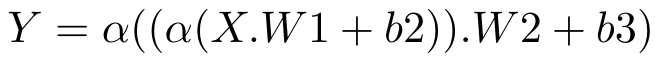
\includegraphics{13.png}
		\caption{Fume Hood}
\end{figure}
\subsection{Source Measuring Unit (SMU)}
\begin{figure}[H]
	\centering
		
		
\includegraphics{14.png}
		\caption{Source Measuring Unit}
\end{figure}
\subsection{Power Supply}
\begin{figure}[H]
	\centering
		
		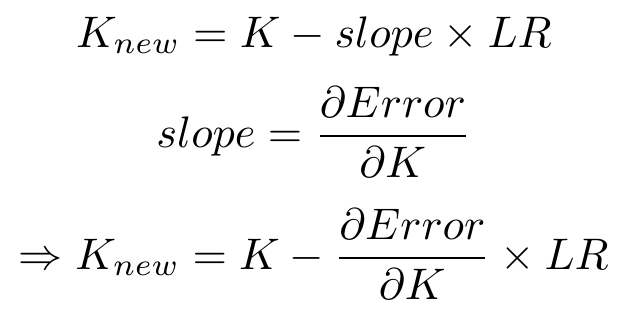
\includegraphics{15.png}
		\caption{Power Supply}
\end{figure}
\subsection{Probe Station}
\begin{figure}[H]
	\centering
		
		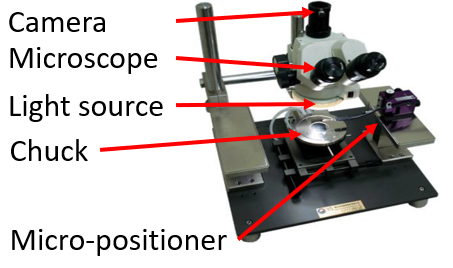
\includegraphics{16.png}
		\caption{Probe Station}
\end{figure}
\subsection{Oscilloscope}
\begin{figure}[H]
	\centering
		
		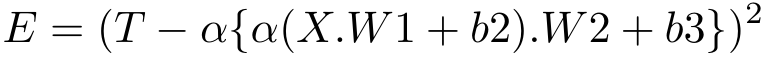
\includegraphics{17.png}
		\caption{Oscilloscope }
\end{figure}
\section{LabView measurement automation}


\section{\label{sec:outline}Outline of the remaining chapters}

The outline of the remaining chapters are as follows. Chapter~\ref{ch:results} provides the results ... 

Physics of Ferromagnetism~\cite{chika97}, Brown~\cite{brown68}             %K
\chapter{Results}
\label{ch:results}


\highlight{I}n this chapter, we provide the results 
\section{Character Recognition Evaluation}
\section{Experimental results after Magnetic Thermal Annealing}
\section{VSM results of Ta/MgO/CoFeB}
\section{FMR results of Ta/MgO/CoFeB}   %K
\chapter{Future Works}
\label{ch:futureworks}

\highlight{I}n this chapter, we will ...
\section{Piezoelectrics}
\section{Electron Beam Lithography}
\section{Block Co-Polymer Lithography}  %K
\cleardoublepage

%%\fancyfoot[C]{\bfseries{A - \thepage}}
%\newpage \pagenumbering{arabic}
%\renewcommand\thepage{A-\arabic{page}}
%\appendix


%\newpage \pagenumbering{arabic}
%\fancyfoot[C]{\bfseries{BIB - \thepage}}
%\renewcommand\thepage{B-\arabic{page}}
\bibliographystyle{unsrt}
%\nocite{*}
\phantomsection
\addcontentsline{toc}{chapter}{Bibliography}
\bibliography{References}
\cleardoublepage

%\phantomsection
%\addcontentsline{toc}{chapter}{List of Publications}
%\include{Publications}  %K

%\newpage \clearpage
%\renewcommand\thepage{}
\phantomsection
\addcontentsline{toc}{chapter}{Vita}
\vspace*{0.5mm}
\begin{center}
\large{Vita}
\end{center}

\vspace*{1cm}
\begin{minipage}[t]{6in}
\setlength{\parindent}{0mm}
Name was born on ... He/She graduated from ...
\end{minipage}
  %K
\clearpage

%\printindex
%\addcontentsline{toc}{chapter}{Index}
%
%\printglossary
%\addcontentsline{toc}{chapter}{Glossary}

\end{document}
